\documentclass{standalone}
\usepackage{tikz}
\usetikzlibrary{patterns, positioning}
\usepackage[sfdefault]{ClearSans} %% option 'sfdefault' activates Clear Sans as the default text font
\usepackage[T1]{fontenc}

\begin{document}
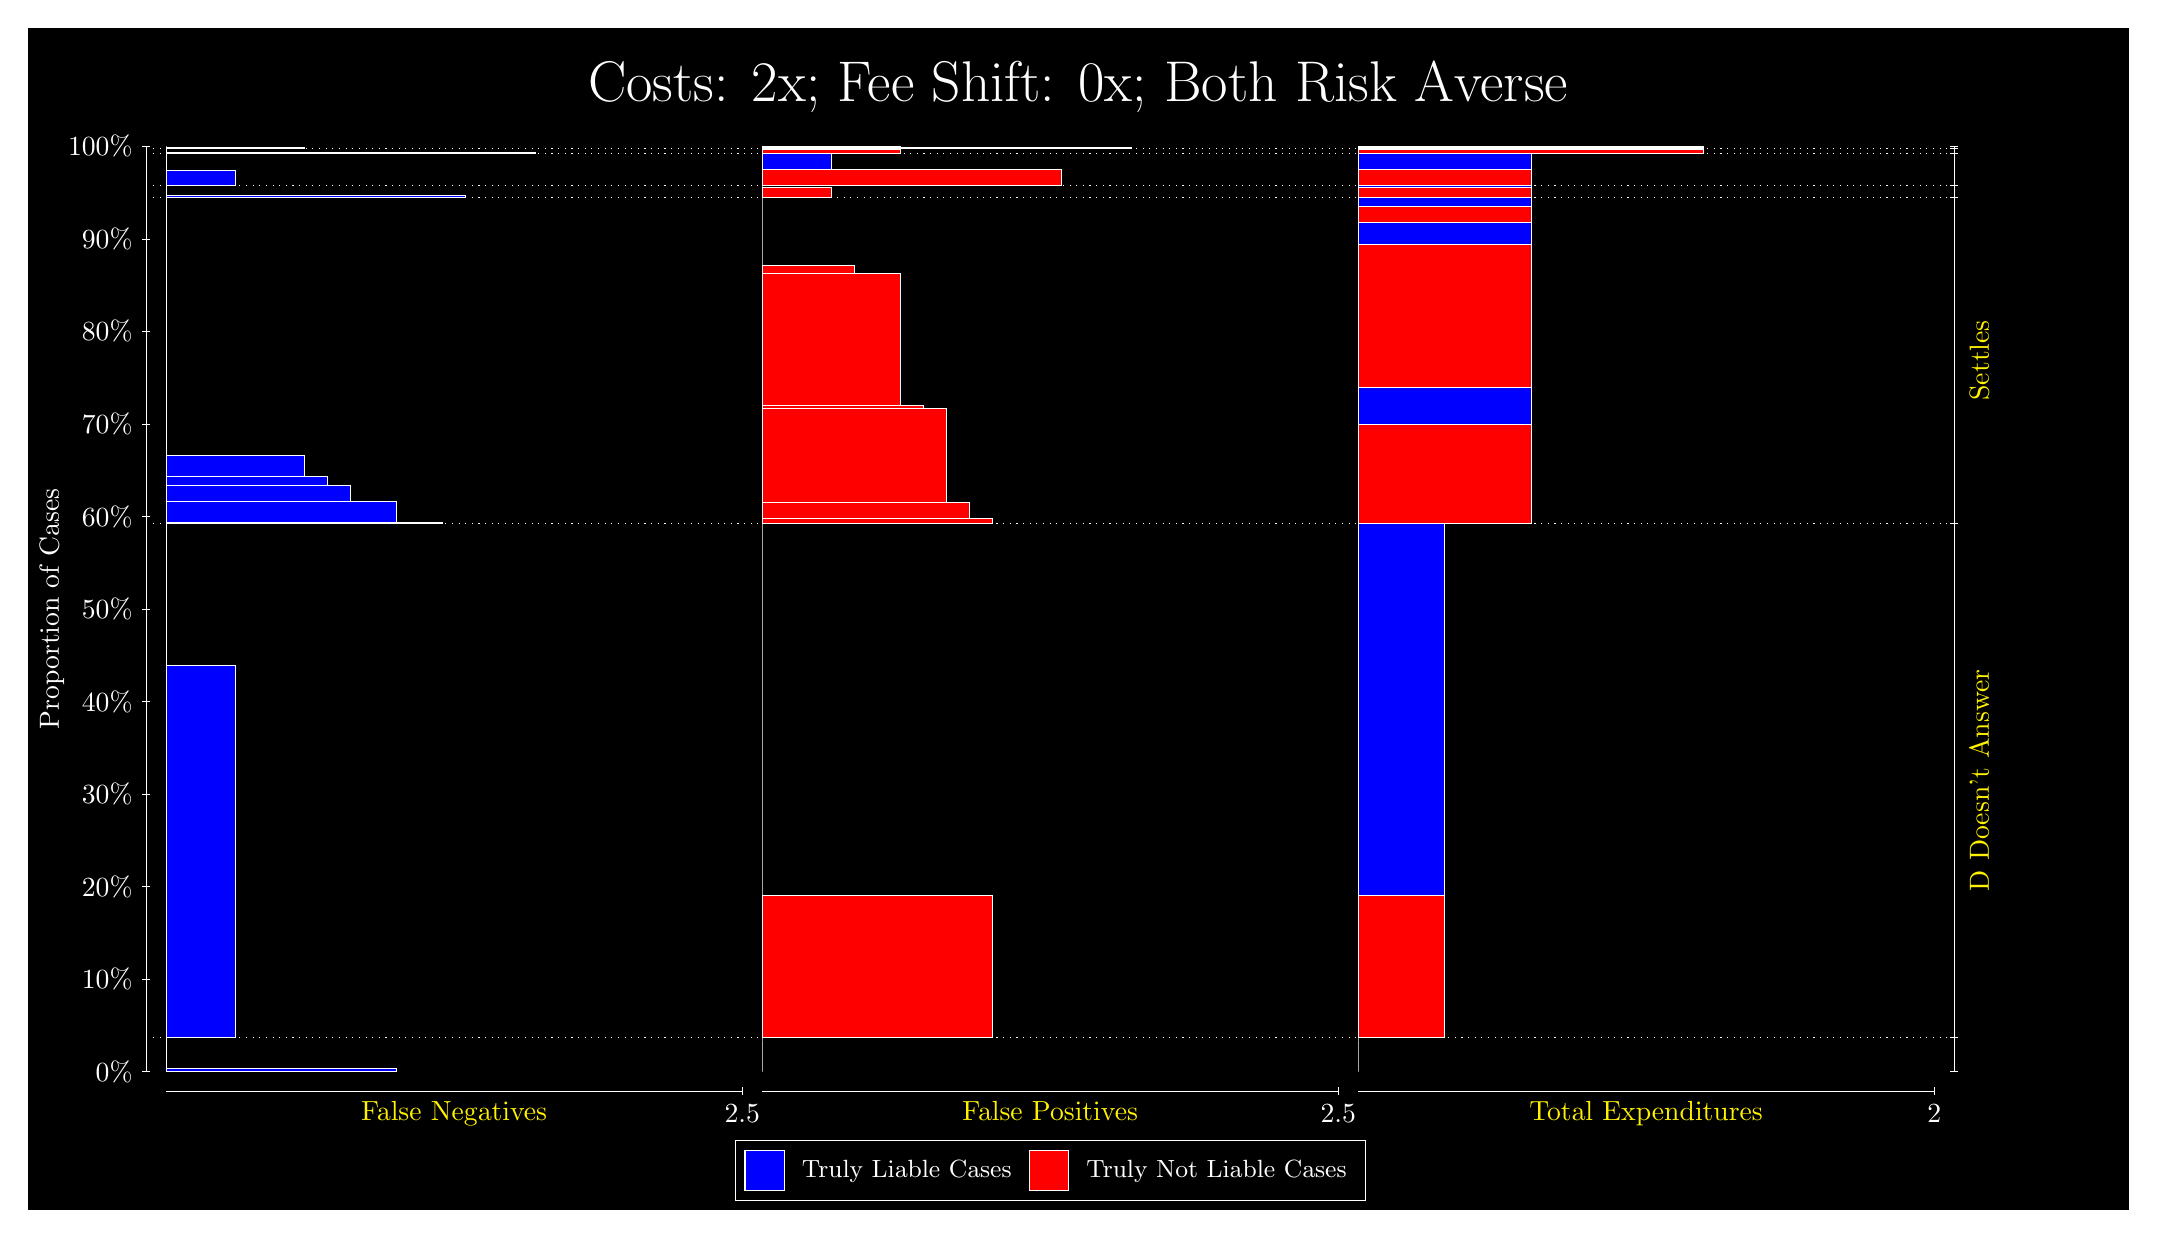
\begin{tikzpicture}
\draw[fill=black] (0,0) rectangle (26.667,15);
\draw[text=white] (0,13.5) rectangle (26.667,15) node[midway] {\huge Costs: 2x; Fee Shift: 0x; Both Risk Averse};
\draw[white, very thin] (1.5,1.75) -- (1.5,13.5);
\node[rotate=90, text=white, anchor=center] at (0.3, 7.625) {Proportion of Cases};
\draw[white, very thin] (1.45,1.75) -- (1.55,1.75);
\node[text=white, anchor=east] at (1.45, 1.75) {0\%};
\draw[white, very thin] (1.45,2.925) -- (1.55,2.925);
\node[text=white, anchor=east] at (1.45, 2.925) {10\%};
\draw[white, very thin] (1.45,4.1) -- (1.55,4.1);
\node[text=white, anchor=east] at (1.45, 4.1) {20\%};
\draw[white, very thin] (1.45,5.275) -- (1.55,5.275);
\node[text=white, anchor=east] at (1.45, 5.275) {30\%};
\draw[white, very thin] (1.45,6.45) -- (1.55,6.45);
\node[text=white, anchor=east] at (1.45, 6.45) {40\%};
\draw[white, very thin] (1.45,7.625) -- (1.55,7.625);
\node[text=white, anchor=east] at (1.45, 7.625) {50\%};
\draw[white, very thin] (1.45,8.8) -- (1.55,8.8);
\node[text=white, anchor=east] at (1.45, 8.8) {60\%};
\draw[white, very thin] (1.45,9.975) -- (1.55,9.975);
\node[text=white, anchor=east] at (1.45, 9.975) {70\%};
\draw[white, very thin] (1.45,11.15) -- (1.55,11.15);
\node[text=white, anchor=east] at (1.45, 11.15) {80\%};
\draw[white, very thin] (1.45,12.325) -- (1.55,12.325);
\node[text=white, anchor=east] at (1.45, 12.325) {90\%};
\draw[white, very thin] (1.45,13.5) -- (1.55,13.5);
\node[text=white, anchor=east] at (1.45, 13.5) {100\%};

\draw[white, very thin] (24.457,1.75) -- (24.457,13.5);
\draw[white, very thin] (24.407,1.75) -- (24.507,1.75);
\node[anchor=west] at (24.407, 1.75) {};
\draw[white, very thin] (24.407,2.1873) -- (24.507,2.1873);
\node[anchor=west] at (24.407, 2.1873) {};
\draw[white, very thin] (24.407,8.7102) -- (24.507,8.7102);
\node[anchor=west] at (24.407, 8.7102) {};
\draw[white, very thin] (24.407,12.854) -- (24.507,12.854);
\node[anchor=west] at (24.407, 12.854) {};
\draw[white, very thin] (24.407,13.006) -- (24.507,13.006);
\node[anchor=west] at (24.407, 13.006) {};
\draw[white, very thin] (24.407,13.406) -- (24.507,13.406);
\node[anchor=west] at (24.407, 13.406) {};
\draw[white, very thin] (24.407,13.471) -- (24.507,13.471);
\node[anchor=west] at (24.407, 13.471) {};
\draw[white, very thin] (24.407,13.5) -- (24.507,13.5);
\node[anchor=west] at (24.407, 13.5) {};

\draw[white, very thin, fill=blue] (1.75,1.75) rectangle (4.6775,1.796);
\draw[white, very thin, fill=red] (1.75,1.796) rectangle (1.75,2.1873);
\draw[white, very thin, fill=blue] (1.75,2.1873) rectangle (2.6283,6.9036);
\draw[white, very thin, fill=red] (1.75,6.9036) rectangle (1.75,8.7102);
\draw[white, very thin, fill=blue] (1.75,8.7102) rectangle (5.2631,8.7256);
\draw[white, very thin, fill=blue] (1.75,8.7256) rectangle (4.6775,8.9869);
\draw[white, very thin, fill=blue] (1.75,8.9869) rectangle (4.3848,8.9973);
\draw[white, very thin, fill=blue] (1.75,8.9973) rectangle (4.092,9.1945);
\draw[white, very thin, fill=blue] (1.75,9.1945) rectangle (3.7993,9.3044);
\draw[white, very thin, fill=blue] (1.75,9.3044) rectangle (3.5065,9.5767);
\draw[white, very thin, fill=red] (1.75,9.5767) rectangle (1.75,12.854);
\draw[white, very thin, fill=blue] (1.75,12.854) rectangle (5.5558,12.876);
\draw[white, very thin, fill=red] (1.75,12.876) rectangle (1.75,13.006);
\draw[white, very thin, fill=blue] (1.75,13.006) rectangle (2.6283,13.201);
\draw[white, very thin, fill=red] (1.75,13.201) rectangle (1.75,13.406);
\draw[white, very thin, fill=blue] (1.75,13.406) rectangle (6.4341,13.421);
\draw[white, very thin, fill=red] (1.75,13.421) rectangle (1.75,13.471);
\draw[white, very thin, fill=blue] (1.75,13.471) rectangle (3.5065,13.486);
\draw[white, very thin, fill=red] (1.75,13.486) rectangle (1.75,13.5);
\draw[white, very thin, fill=red] (9.3189,1.75) rectangle (9.3189,2.1413);
\draw[white, very thin, fill=blue] (9.3189,2.1413) rectangle (9.3189,2.1873);
\draw[white, very thin, fill=red] (9.3189,2.1873) rectangle (12.246,3.9938);
\draw[white, very thin, fill=blue] (9.3189,3.9938) rectangle (9.3189,8.7102);
\draw[white, very thin, fill=red] (9.3189,8.7102) rectangle (12.246,8.7768);
\draw[white, very thin, fill=red] (9.3189,8.7768) rectangle (11.954,8.9804);
\draw[white, very thin, fill=red] (9.3189,8.9804) rectangle (11.661,10.176);
\draw[white, very thin, fill=red] (9.3189,10.176) rectangle (11.368,10.214);
\draw[white, very thin, fill=red] (9.3189,10.214) rectangle (11.075,11.891);
\draw[white, very thin, fill=red] (9.3189,11.891) rectangle (10.49,11.987);
\draw[white, very thin, fill=blue] (9.3189,11.987) rectangle (9.3189,12.854);
\draw[white, very thin, fill=red] (9.3189,12.854) rectangle (10.197,12.984);
\draw[white, very thin, fill=blue] (9.3189,12.984) rectangle (9.3189,13.006);
\draw[white, very thin, fill=red] (9.3189,13.006) rectangle (13.125,13.211);
\draw[white, very thin, fill=blue] (9.3189,13.211) rectangle (10.197,13.406);
\draw[white, very thin, fill=red] (9.3189,13.406) rectangle (11.075,13.457);
\draw[white, very thin, fill=blue] (9.3189,13.457) rectangle (9.3189,13.471);
\draw[white, very thin, fill=red] (9.3189,13.471) rectangle (14.003,13.485);
\draw[white, very thin, fill=blue] (9.3189,13.485) rectangle (11.075,13.5);
\draw[white, very thin, fill=red] (16.888,1.75) rectangle (16.888,2.1413);
\draw[white, very thin, fill=blue] (16.888,2.1413) rectangle (16.888,2.1873);
\draw[white, very thin, fill=red] (16.888,2.1873) rectangle (17.986,3.9938);
\draw[white, very thin, fill=blue] (16.888,3.9938) rectangle (17.986,8.7102);
\draw[white, very thin, fill=red] (16.888,8.7102) rectangle (19.083,9.9725);
\draw[white, very thin, fill=blue] (16.888,9.9725) rectangle (19.083,10.442);
\draw[white, very thin, fill=red] (16.888,10.442) rectangle (19.083,12.253);
\draw[white, very thin, fill=blue] (16.888,12.253) rectangle (19.083,12.54);
\draw[white, very thin, fill=red] (16.888,12.54) rectangle (19.083,12.744);
\draw[white, very thin, fill=blue] (16.888,12.744) rectangle (19.083,12.854);
\draw[white, very thin, fill=red] (16.888,12.854) rectangle (19.083,12.984);
\draw[white, very thin, fill=blue] (16.888,12.984) rectangle (19.083,13.006);
\draw[white, very thin, fill=red] (16.888,13.006) rectangle (19.083,13.211);
\draw[white, very thin, fill=blue] (16.888,13.211) rectangle (19.083,13.406);
\draw[white, very thin, fill=red] (16.888,13.406) rectangle (21.279,13.457);
\draw[white, very thin, fill=blue] (16.888,13.457) rectangle (21.279,13.471);
\draw[white, very thin, fill=red] (16.888,13.471) rectangle (21.279,13.485);
\draw[white, very thin, fill=blue] (16.888,13.485) rectangle (21.279,13.5);
\draw[white, dotted] (1.5,2.1873) -- (24.457,2.1873);
\draw[white, dotted] (1.5,8.7102) -- (24.457,8.7102);
\draw[white, dotted] (1.5,12.854) -- (24.457,12.854);
\draw[white, dotted] (1.5,13.006) -- (24.457,13.006);
\draw[white, dotted] (1.5,13.406) -- (24.457,13.406);
\draw[white, dotted] (1.5,13.471) -- (24.457,13.471);
\draw[white, very thin] (1.75,1.5) -- (9.0689,1.5);
\node[text=yellow, anchor=north] at (5.4094, 1.5) {False Negatives};
\draw[white, very thin] (9.0689,1.45) -- (9.0689,1.55);
\node[text=white, anchor=north] at (9.0689, 1.45) {2.5};

\draw[white, very thin] (9.3189,1.5) -- (16.638,1.5);
\node[text=yellow, anchor=north] at (12.978, 1.5) {False Positives};
\draw[white, very thin] (16.638,1.45) -- (16.638,1.55);
\node[text=white, anchor=north] at (16.638, 1.45) {2.5};

\draw[white, very thin] (16.888,1.5) -- (24.207,1.5);
\node[text=yellow, anchor=north] at (20.547, 1.5) {Total Expenditures};
\draw[white, very thin] (24.207,1.45) -- (24.207,1.55);
\node[text=white, anchor=north] at (24.207, 1.45) {2};


\node[text=yellow, centered, rotate=90] at (24.777, 5.4487) {D Doesn't Answer};
\node[text=yellow, centered, rotate=90] at (24.777, 10.782) {Settles};





\draw (12.978300999999998,1.5) node[draw=none] (baseCoordinate) {};
\begin{scope}[align=center]
        \matrix[scale=0.5, draw=white, below=0.5cm of baseCoordinate, nodes={draw}, column sep=0.1cm]{
            \node[rectangle, draw, minimum width=0.5cm, minimum height=0.5cm, fill=blue] {}; &
            \node[draw=none, font=\small, text=white] (B) {Truly Liable Cases}; &
            \node[rectangle, draw, minimum width=0.5cm, minimum height=0.5cm, fill=red] {}; &
            \node[draw=none, font=\small, text=white] (B) {Truly Not Liable Cases}; \\
            };
\end{scope}

\end{tikzpicture}
\end{document}